% !TeX root = ../report_project_2stage_OTA.tex

\section{Ideal Two-Stage Model}

An ideal small-signal model is first used to verify the analytical
two-stage design independently of MOS transistor parasitics.

Each gain stage is represented by a voltage-controlled current source
and its corresponding output resistance. The model parameters are
directly obtained from the first-order transistor sizing:

\[
g_{m1} = 5~\mu\mathrm{S},
\qquad
R_{\mathrm{out1}} = 29.7~\mathrm{M}\Omega
\]

and

\[
g_{m2} = 54.4~\mu\mathrm{S},
\qquad
R_{\mathrm{out2}} = 2.81~\mathrm{M}\Omega.
\]

The two stages are compensated using

\[
C_{\mathrm{MILLER}} = 0.8~\mathrm{pF}.
\]

No additional internal capacitance is introduced at this stage.
The objective is to isolate the behavior predicted by the first-order
two-stage model. The external load capacitance is applied from the
testbench.

\begin{figure}[ht]
    \centering
    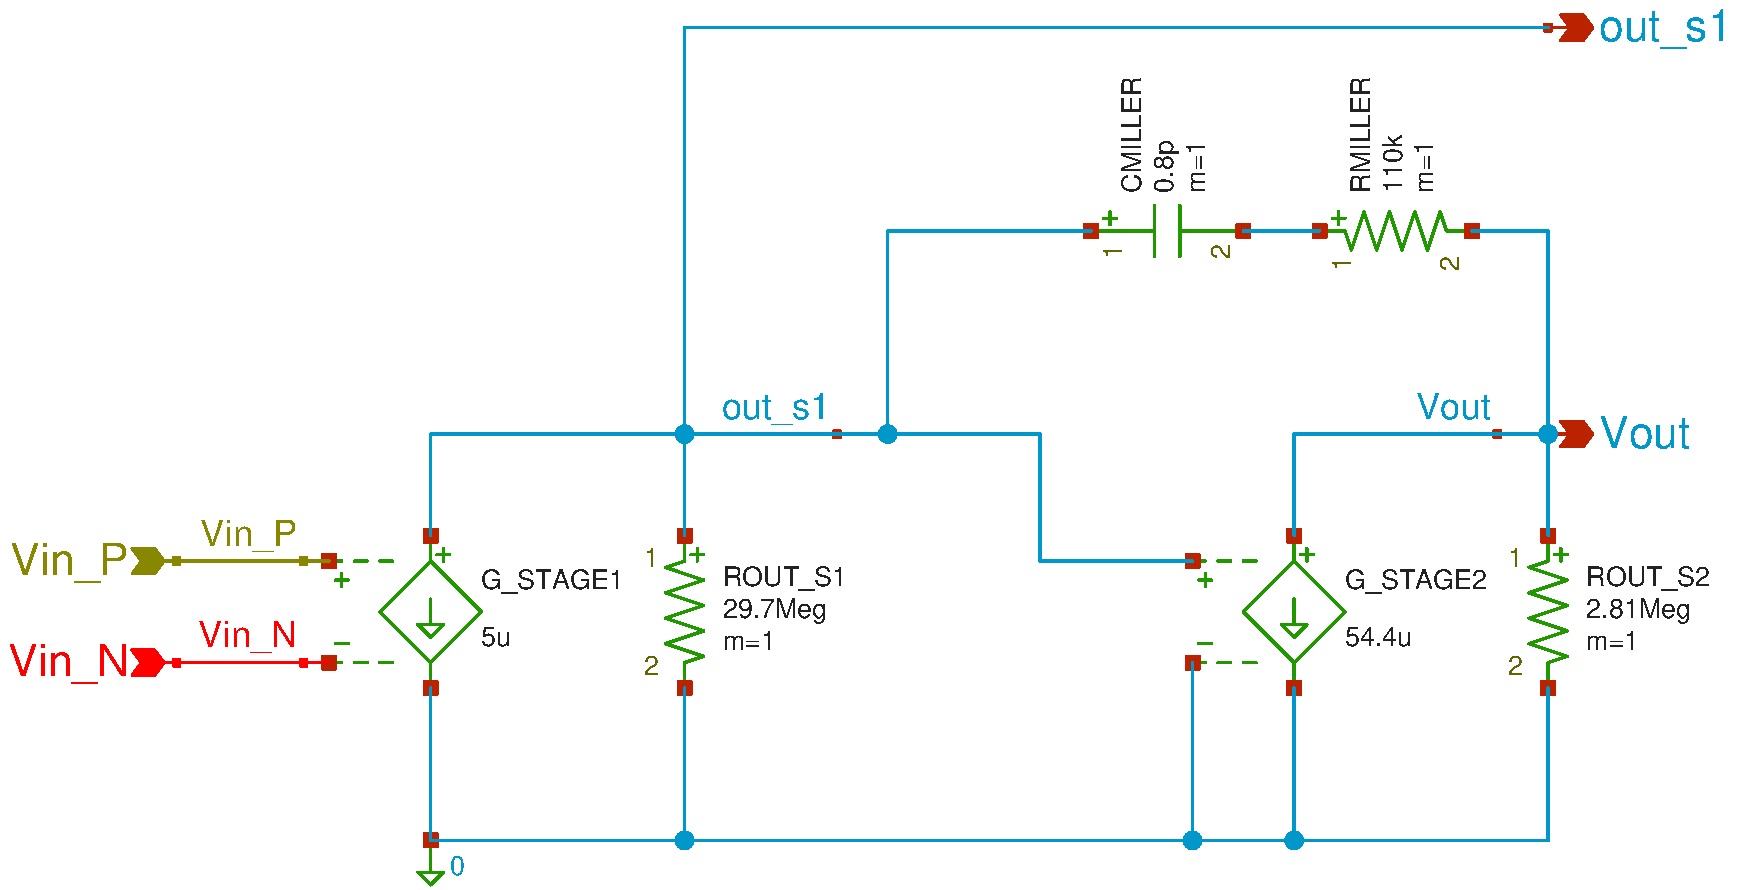
\includegraphics[width=\textwidth]
    {figures/ideal/schematics/ota_2stage_ideal.pdf}
    \caption{Ideal two-stage OTA model using transconductance stages,
    calculated output resistances and Miller compensation.}
    \label{fig:ideal_ota_schematic}
\end{figure}

\subsection{Nominal AC Response}

The initial AC simulation uses

\[
C_L = 2~\mathrm{pF}.
\]

The simulated low-frequency gain is

\[
A_0 = 87.1~\mathrm{dB},
\]

while the unity-gain frequency is

\[
f_{\mathrm{UGF}} = 966.7~\mathrm{kHz}.
\]

The phase at unity gain is

\[
\phi(f_{\mathrm{UGF}}) = -107.6^\circ,
\]

corresponding to a phase margin of

\[
\boxed{PM = 72.4^\circ}.
\]

The ideal model therefore reproduces the analytical gain and bandwidth
predictions closely while providing comfortable margin relative to the
$60^\circ$ stability target.

\subsection{Load-Capacitance Sensitivity}

The load capacitance was increased from the nominal value of
$2~\mathrm{pF}$ to the specified maximum value of $4~\mathrm{pF}$,
without modifying the OTA parameters.

The resulting AC performance is summarized in
Table~\ref{tab:ideal_load_sweep}.

\begin{table}[ht]
    \centering
    \caption{Ideal-model AC performance versus load capacitance.}
    \label{tab:ideal_load_sweep}
    \begin{tabular}{lccc}
        \hline
        $C_L$ & DC gain & UGF & Phase margin \\
        \hline
        2 pF & 87.1 dB & 966.7 kHz & $72.4^\circ$ \\
        4 pF & 87.1 dB & 912.0 kHz & $62.5^\circ$ \\
        \hline
    \end{tabular}
\end{table}

As expected, the low-frequency gain is essentially unaffected by the
capacitive load. The increased load capacitance lowers the non-dominant
pole and therefore reduces the phase margin.

At $C_L=4~\mathrm{pF}$, the model retains approximately $62.5^\circ$ of
phase margin and therefore still satisfies the initial $60^\circ$
stability target, although with limited additional margin.

\subsection{Miller Zero Compensation}

Without a series compensation resistor, the Miller feedforward path
introduces a right-half-plane zero approximately located at

\[
f_{z,\mathrm{RHP}}
\approx
\frac{g_{m2}}
     {2\pi C_{\mathrm{MILLER}}}
\approx
10.8~\mathrm{MHz}.
\]

For a series Miller resistor, the first-order zero location depends on

\[
R_{\mathrm{MILLER}}
-
\frac{1}{g_{m2}}.
\]

For

\[
R_{\mathrm{MILLER}}
\approx
\frac{1}{g_{m2}}
\approx
18.4~\mathrm{k}\Omega,
\]

the RHP zero is approximately pushed to infinity. At the maximum
$4~\mathrm{pF}$ load, this increases the phase margin from
$62.5^\circ$ to $67.4^\circ$ with negligible bandwidth penalty.

A larger resistance creates a left-half-plane zero. To compensate the
phase lag introduced by the non-dominant output pole, the zero was
placed approximately around

\[
f_{p2}
\approx
\frac{g_{m2}}
     {2\pi C_L}
\approx
2.2~\mathrm{MHz}.
\]

This gives an initial resistor estimate of approximately

\[
R_{\mathrm{MILLER}}
\approx
110~\mathrm{k}\Omega.
\]

The resulting LHP zero provides phase lead around the second-pole
frequency, making the open-loop response behave approximately as a
single-pole system around unity gain without increasing
$C_{\mathrm{MILLER}}$.

\begin{table}[ht]
    \centering
    \caption{Ideal-model compensation and load study.}
    \label{tab:ideal_compensation}
    \begin{tabular}{lcccc}
        \hline
        $C_L$ & $R_{\mathrm{MILLER}}$ & DC gain & UGF & PM \\
        \hline
        2 pF & 0 $\Omega$     & 87.1 dB & 966.7 kHz & $72.4^\circ$ \\
        4 pF & 0 $\Omega$     & 87.1 dB & 912.0 kHz & $62.5^\circ$ \\
        4 pF & 18.4 k$\Omega$ & 87.1 dB & 909.1 kHz & $67.4^\circ$ \\
        4 pF & 110 k$\Omega$  & 87.1 dB & 985.2 kHz & $90.1^\circ$ \\
        \hline
    \end{tabular}
\end{table}

\begin{figure}[ht]
    \centering
    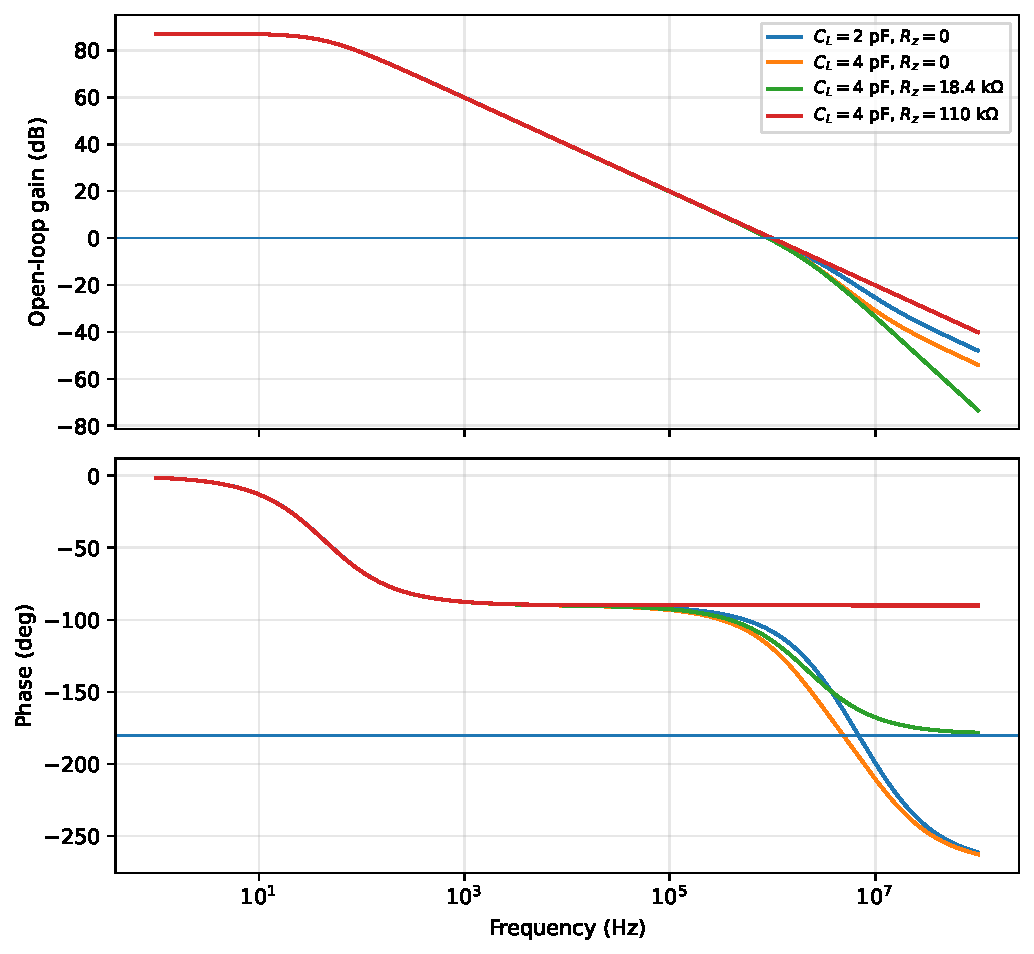
\includegraphics[width=\textwidth]
    {figures/ideal/ac/ideal_ac_compensation_comparison.pdf}
    \caption{Ideal open-loop response showing the effect of load
    capacitance and Miller zero compensation.}
    \label{fig:ideal_ac_compensation}
\end{figure}

The $110~\mathrm{k}\Omega$ case demonstrates the intended pole-zero
compensation mechanism particularly clearly: the LHP zero approximately
counteracts the phase lag of the second pole around the relevant
frequency range.

This value is therefore retained as the initial compensation-resistor
estimate for the transistor-level design. Its optimum value is expected
to shift once transistor parasitics and additional high-frequency poles
are introduced.
